\documentclass[12pt]{article}

\usepackage[dvips,letterpaper,margin=0.75in,bottom=0.5in]{geometry}
\usepackage{cite}
\usepackage{slashed}
\usepackage{graphicx}
\usepackage{amsmath}

\begin{document}

\title{Arduino Audio Digital Spectrum Analyzer}
\author{Michael Mulhearn}

\maketitle

\section{Introduction}

In this lab, we will construct an audio spectrum analyzer.  The output from a microphone and amplifier, contained on a integrated circuit, will be digitized by an Arduino microprocessor using the ADC in free-running mode and stored in a buffer.  When the buffer is full, the data will be uploaded to your PC over the serial port for Fourier analysis.  The PC will be driving the data collection, requesting the samples from the Arduino via a custom hardware driver interface.

In this lab, you will learn about hardware integration.  Most interesting technical feats are broken down into manageable components, often designed by different teams.  Someday, you may have the challenging job of integrating your colleagues components together into a working system.   The system that your colleagues (aka me) will provide are:
\begin{itemize}
\item A microphone IC, with $5~\rm V$ output, specifically designed for use with the Arduino.
\item An Arduino Digital Scope sketch (Scope), which will be used to sample the microphone.
\item An Arduino serial data service sketch (SerialDataService) which, upon request over the serial interface, fills a buffer with fake data and reports it on the serial interface.
\item A scientific python driver (serial\_driver\.py), which requests data from the serial data service and plots it.
\item A Scientific Python code snippet demonstrating the scientific python Periodogram feature, which reports the magnitude of the Fourier coefficients for a discreetly sampled waveform.
\end{itemize}
Your job will be to put all of these working components\footnote{Here we differ from the real world, where often you get components that don't work as intended!} together and construct an audio spectrum analyzer, which you can use to check the tuning of a guitar. 

Here's one way to go about the integration:  
\begin{itemize}
\item First, I would get the microphone working with the digital scope example code, then I would put this aside for a bit.
\item Next, I would get the serial data service sketch working with the scientific python code snippet.
\item Next, I would modify the python driver code to calculate and plot the periodogram, and test it using the fake data from the serial data service... it's much easier to debug on test patterns!
\item Last, I would modify the serial data service to use the microphone data, by importing the relevant code from the Scope sketch.  (I would keep the ability to use test patterns instead, in case debugging is needed!)
\item If I had time, I would provide the Periodogram that results from averaging several samples, which should boost the signal to noise ratio.
\end{itemize}
The following sections will describe the theory behind the Periodogram, and the inner workings of the individual components.  Putting it all together will be left to you!

\section{Fourier Series for Discreet Data}

To tune a guitar, for example, we need to determine the frequency spectrum of sound when a string is plucked.   Conceptually, the guitar provides $f(t)$ and we simply wish to calculate the Fourier transform $\widetilde{f}(\omega)$.  The start time is arbitrary, so the phase is meaningless, and so in fact we need only 
$|\widetilde{f}(\omega)|^2$.

But we do not have a continuous function $f(t)$   Instead, we will be sampling the microphone at discrete intervals separated by the sampling period $\tau$.  We have limited time and buffer space, so we will only sample during a limited period $T$.  Instead of the Fourier Transform, we will be calculating the discrete Fourier series.

Our time series data will consist of $n$ microphone values $x_j$, collected during a time interval of duration $T = n\tau$, and approximately evenly spaced.    Let's start with the Fourier Series for a function of time with period $T$.  In this case, neglecting the overall normalization, which we don't care about, the formula for calculating the Fourier coefficients is:
\begin{eqnarray*}
A_m &=&  \int_{-\frac{T}{2}}^{\frac{T}{2}} 
f(x) \cos\left(\frac{2\pi m}{T} \, t \right) \, dt \\
B_m &=& \int_{-\frac{T}{2}}^{\frac{T}{2}} 
f(x) \sin\left(\frac{2\pi m}{T} \, t \right) \, dt
\end{eqnarray*}
we can describe our discrete data sample, however, as:
\begin{equation*}
f(t) \to \sum_{i=0}^n \delta(t-i\tau) x_i
\end{equation*}
that is, it is zero everywhere but at the $n$ sample points, each at location $i\tau$ in time, where the value is $x_i$.
The delta function replaces the integrals above with sums, and the coefficients are now given by:
\begin{eqnarray*}
A_m &=&  \sum_{i=0}^n x_i  \cos\left(\frac{2\pi m}{n} \, i \right) \\
B_m &=&  \sum_{i=0}^n x_i  \sin\left(\frac{2\pi m}{n} \, i \right) \\
\end{eqnarray*}
Recall that the frequency associated with each $m$ is $f_m = m / T$.  Therefore, our lowest frequency (for $m=1$) is $f=1/T$.  From the Nyquist theorem, the highest frequency we can reliably sample is one half the sampling rate ($1/nT$) and therefore we'll have Fourier series coefficients for the frequencies:
\begin{displaymath}
f_m = \frac{m}{T} \; \; \; {\rm for} \; m=1,2,3,\ldots,\frac{n}{2}
\end{displaymath}

There are more computation efficient ways to calculate the Discreet Fourier Series which are known collectively as the Fast Fourier Transform.   But we won't need to understand these algorithms as they merely reproduce the conceptually simple computation above (though much much faster).  We'll be using the periodogram feature, which reports $\sqrt{A_m^2 + B_m^2}$ for each $f_m$.

Now let's look at particular our particular case.  With the Arduino in free running mode, the ADC sample rate is $76.9~\rm kHz$ which puts the Nyquist frequency at $33~\rm kHz$.  Any signal above this frequency would lead to aliasing.  Fortunately, this is well above the audio range and the microphone acts as a low-pass filter (see Fig.~\ref{fig:freq} below), eliminating any risk of aliasing from higher frequency signals.

There's enough room in the Arduino for a 1500 byte buffer.  Therefore, our period for signal collection is 
{19.5~\rm ms}.  Our lowest frequency (for $m=1$) is $51.26~\rm Hz$ and our next lowest (for $m=2$) is $102.5~\rm Hz$.   That is actually pretty poor resolution for tuning a guitar, but we'll live with it for now.  A way around this limitation using a digital low pass filter is discussed in the Improvements section.

\section{Microphone IC}

The microphone IC (Fig.~\ref{fig:mic} includes a microphone and a gain 60 pre-amplifier.  This IC is designed for use with Arduino and is very convenient.  You simply connect VCC to $5~\rm V$, GND to Arduino ground, and AUD is audio output in the $0$ to $5~\rm V$ range, suitable for sampling with an analog input.

To test your microphone initially, connect VCC and GND, but measure AUD with your scope.  Whistling should produce a decent sine wave, or find a fixed tone generator online.

\begin{figure}[htbp]
\begin{center}
{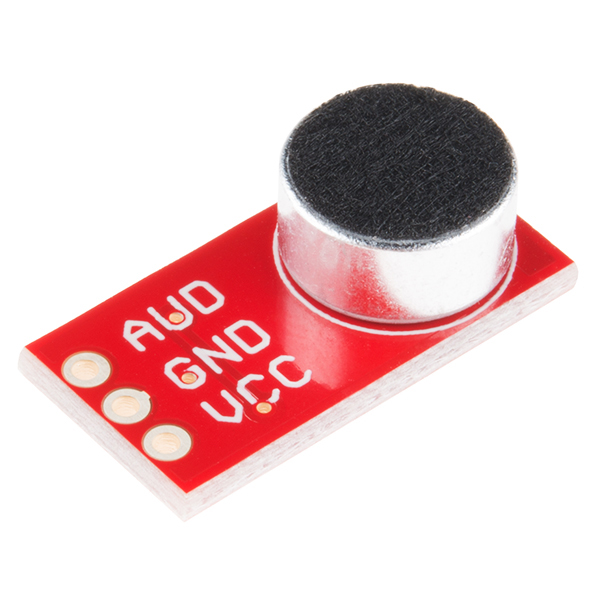
\includegraphics[width=0.20\textwidth]{figs/mic.jpg}}
\end{center}
\caption{\label{fig:mic} The microphone, with preamplifier (not shown) on the underside of the IC.}
\end{figure}

\begin{figure}[htbp]
\begin{center}
{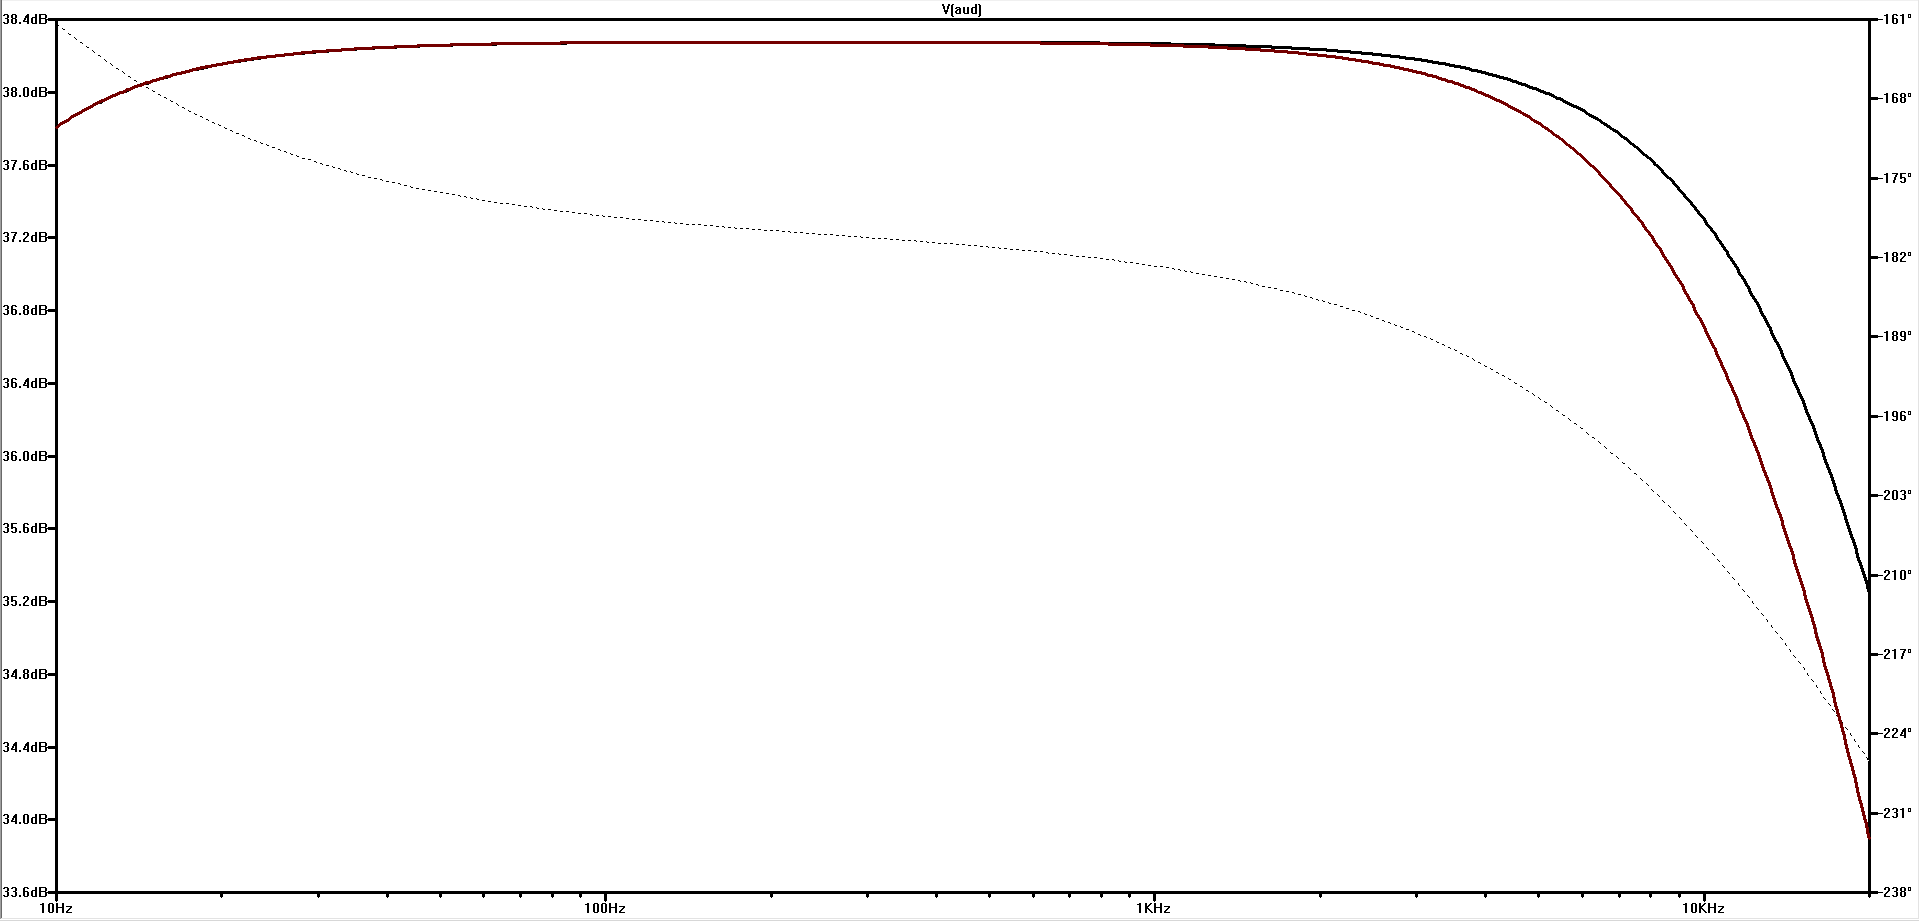
\includegraphics[width=0.75\textwidth]{figs/freq.png}}
\end{center}
\caption{\label{fig:freq} Frequency response of the microphone IC.}
\end{figure}

\section{Scope Sketch}

The scope sketch is much like it was for the Arduino Digital Sketch lab (with a few minor improvements developed during that lab).  There's a section for configuring the ADC for free-running mode using low-level Arduino hardware drive code in the setup: 
\begin{verbatim}
 ADCSRA = 0;             // clear ADCSRA register
 ADCSRB = 0;             // clear ADCSRB register
 ADMUX |= (adc & 0x07);    // set A(adc) analog input pin
 ADMUX |= (1 << REFS0);  // set reference voltage
 ADMUX |= (1 << ADLAR);  // left align ADC value to 8 bits from ADCH register
 // sampling rate is [ADC clock] / [prescaler] / [conversion clock cycles]
 // for Arduino Uno ADC clock is 16 MHz and a conversion takes 13 clock cycles
 ADCSRA |= (1 << ADPS2);                     // 16 prescaler for 76.9 KHz
 ADCSRA |= (1 << ADATE); // enable auto trigger
 ADCSRA |= (1 << ADIE);  // enable interrupts when measurement complete
 ADCSRA |= (1 << ADEN);  // enable ADC
 ADCSRA |= (1 << ADSC);  // start ADC measurements
\end{verbatim}
The {\tt adc} variable specifies which analog input to digitize.  It is set to 0 in the sketch.

There is also the all-important interrupt service routine, for processing the samples:
\begin{verbatim}
ISR(ADC_vect){
  if (isamp < max_samples){
    buf[isamp]=ADCH;
    isamp++;      
  }
}    
\end{verbatim}
For this lab, there is no need to implement a trigger, as we do not care about the phase of the waveform.
If you connect the microphone IC to the Arduino and whistle, you should observe a decent sine wave, as in Fig.~\ref{fig:whistle}.

\begin{figure}[htbp]
\begin{center}
{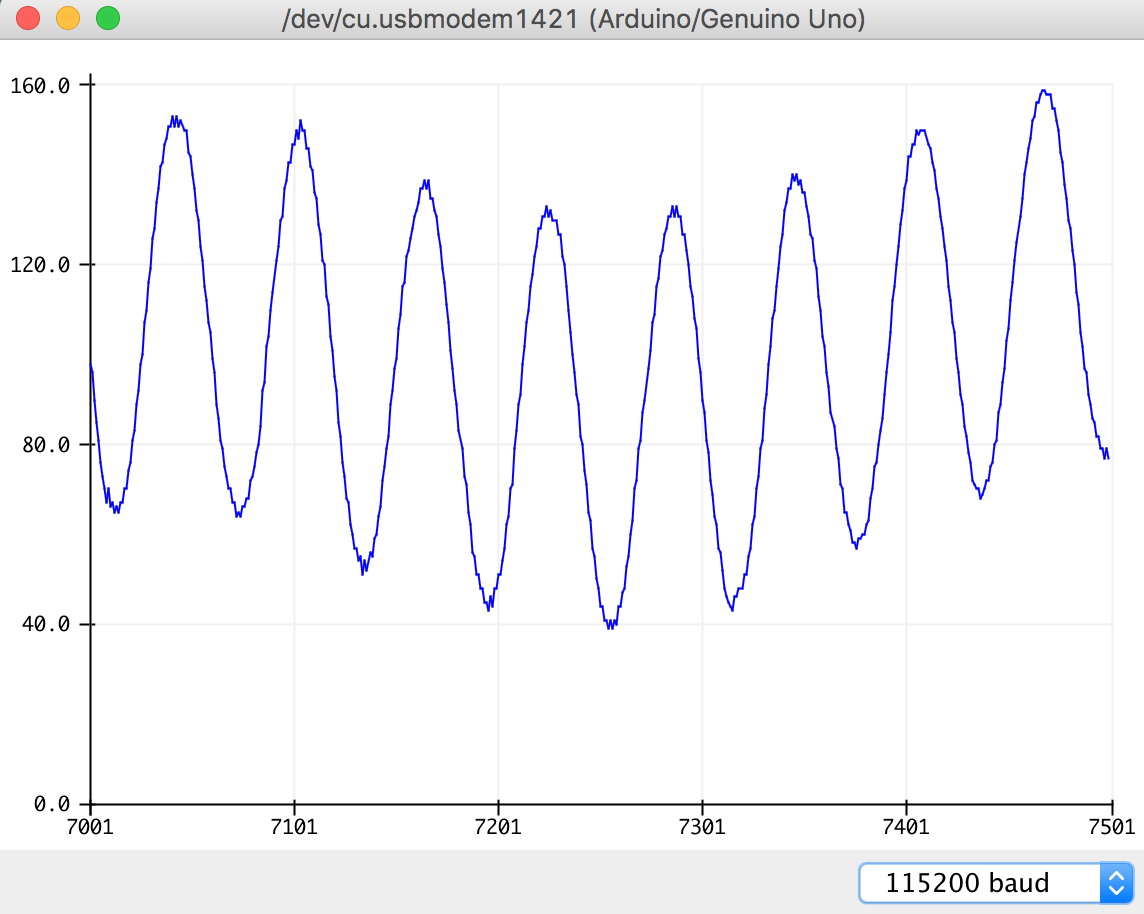
\includegraphics[width=0.75\textwidth]{figs/whistle.png}}
\end{center}
\caption{\label{fig:whistle} A whistle.}
\end{figure}

\section{Serial Data Service Sketch}

Upon request over the the serial interface, the Serial Data Service sketch fills a buffer with a sine wave test pattern and reports it over the serial interface.

The driver interface uses the special function {\tt serialEvent()}.  This function is called after the loop function exits only if new serial data is available at the input:
\begin{verbatim}
void serialEvent() {
  delay(1000);
  char inChar = (char) Serial.read();
  if (inChar == 'a'){
      nruns = (int) Serial.parseInt();
      dt = (int) Serial.parseInt();        
      acquire = 1;
      digitalWrite(led, HIGH);
      isamp = 0;
  }
  while(Serial.available()){
    char inChar = (char) Serial.read();  
  }
  //Serial.println(param_n);
  //Serial.println(param_t);
}
\end{verbatim}
Here we check for our one implemented driver command acquire and two parameters.  The first parameter ({\tt nruns} specifies how many complete wave forms should be send back for this acquire command.  The second parameter {\tt dt} is an example timing parameter.   The acquire command is send as the single letter "a" followed by integer values for the two parameters, which should be both one, at least initially.
Upon receiving this command on the serial interface, the variable {\tt acquire} is set to 1, and the loop function begins filling the buffer, printing it to the serial interface when full.
\begin{verbatim}
void loop() {    
  fill_buffer_with_test_pattern();
  
  if (acquire & (isamp == max_samples)) {
    write_buffer_to_serial_port();
    isamp = 0;    
    count++;
  }

  if (count >= nruns){
    acquire = false;
    digitalWrite(led, LOW);
  }
}
\end{verbatim}
The output to the serial interface starts with a simple ``header" specifying the number of samples in each waveform {\tt max\_samples} and the number of waveforms that will be sent (one for now). 
\begin{verbatim}
void write_buffer_to_serial_port(){
    // write header only for the first sample:
    if (count==0){
      Serial.println(max_samples);
      Serial.println(nruns);
    }
    // write payload:
    for(int i=0; i<max_samples; i++){
      char line[100];
      sprintf(line, "%d %d", i*dt, buf[i]);
      Serial.println(line);
      Serial.flush();
    }
}
\end{verbatim}


You can test out the serial driver interface by hand in the Serial Interface by sending the ascii command "a 1 1" as in Fig.~\ref{fig:send}.  The reply from the Arduino is in  Fig.~\ref{fig:reply}.

\begin{figure}[htbp]
\begin{center}
{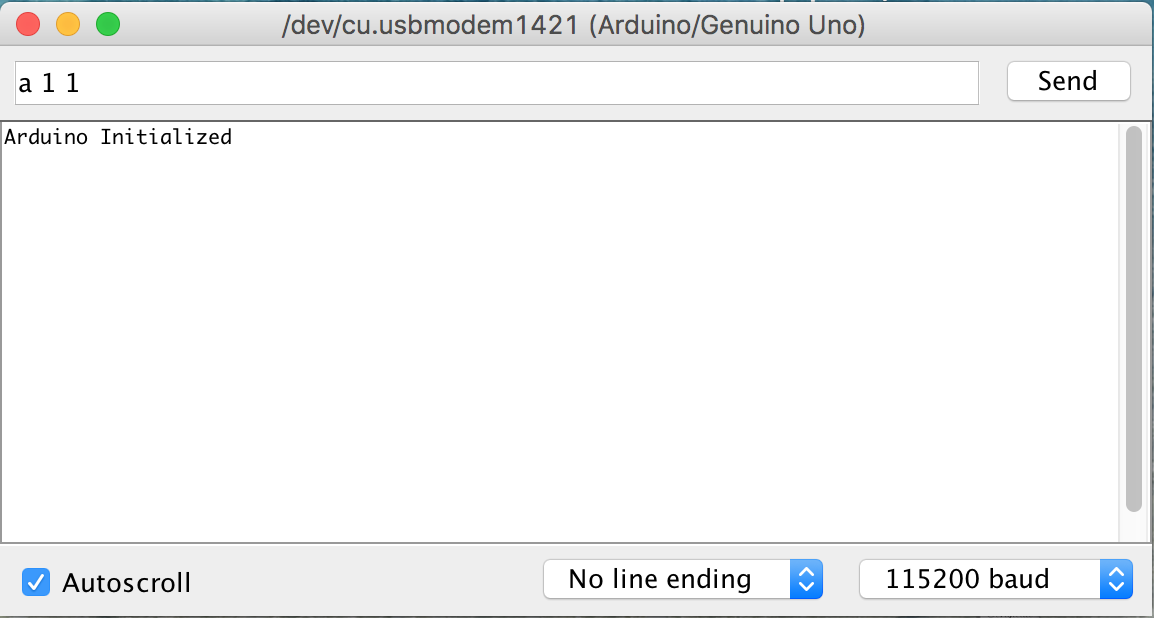
\includegraphics[width=0.75\textwidth]{figs/send.png}}
\end{center}
\caption{\label{fig:send} Sending the acquire command .}
\end{figure}

\begin{figure}[htbp]
\begin{center}
{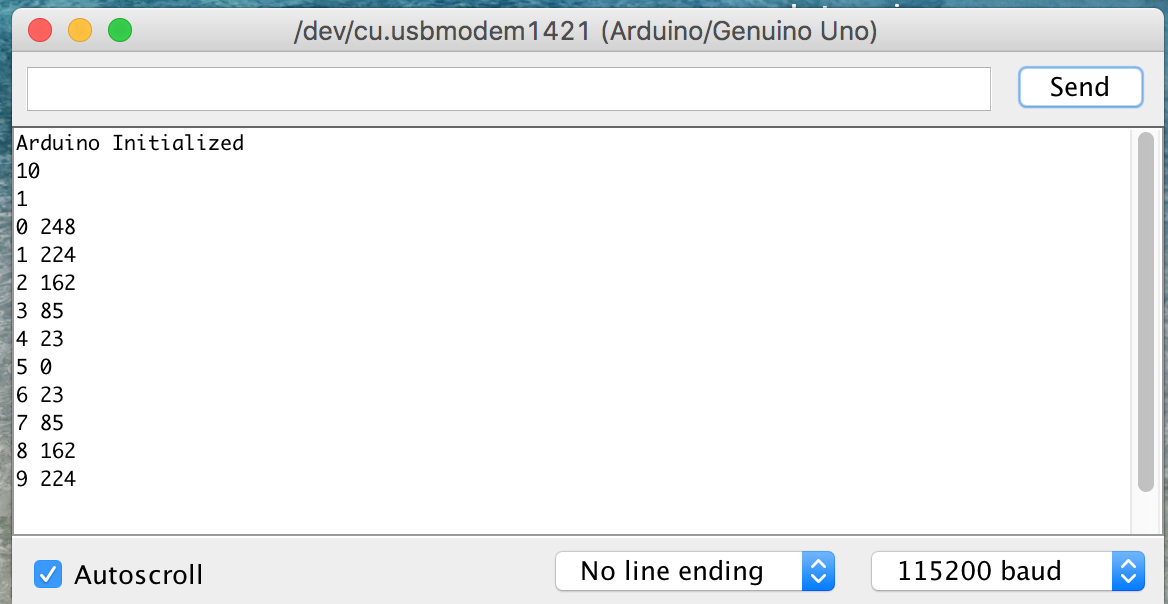
\includegraphics[width=0.75\textwidth]{figs/reply.png}}
\end{center}
\caption{\label{fig:reply} The Arduino reply.}
\end{figure}
The buffer size ({\tt max\_samples} is set to ten initially, to avoid overwhelming you with output when testing in the serial port by hand.  Once you have this under control, you can increase the buffer size by setting {\tt max\_samples} to 1500. 

\section{Python Serial Driver Code}

?he python serial driver code will prompt you for the serial port that the Arduino is located on.  If you get tired of being prompted for this, you can replace the prompt with a hard coded value:
\begin{verbatim}
#SERIAL_PORT="COM4"                                                                                                     
#SERIAL_PORT="/dev/cu.usbmodem1421"                                                                                     
SERIAL_PORT=raw_input("Enter the serial port for the Arduino (e.g. COM4):  ")
\end{verbatim}
The important part of this code is the interaction with the Arduino over the serial port:
\begin{verbatim}
    ser.write("a {1:d} {1:d}".format(nrun, dt))
    # first line is the length of the payload:                                                                          
    nsamp = int(ser.readline().strip())
    nrun  = int(ser.readline().strip())

    xl = np.zeros((nrun,nsamp), dtype=float)
    yl = np.zeros((nrun,nsamp), dtype=float)
    print "receiving payload from Arduion of length ", nsamp, " x ", nrun, "\n";

    for i in range(nrun):
        for j in range(nsamp):
            str = ser.readline().strip()
            # print str                                                                                                 
            x,y = str.split()
            if ((i<5) and (j<5)):
                print "x: ", x, "y: ", y
            xl[i][j] = x;
            yl[i][j] = y;
    ser.close()
\end{verbatim}
Here it sends the acquire command, then reads the Arduino reply saving the results to arrays {\tt x} (sample number) and {\tt y} (waveform).  The arrays are 2D because the code already handles requesting more than one waveform at once.  To start, just use {\tt x[0]} and {\tt y[0]}. 

You shouldn't have to change any of the code before the arrays are filled.  You only have to change how the arrays are processed and plotted.  As currently implemented, the code simply plots the waveform as in Fig.~\ref{fig:wave}.  You'll want to replace this with the periodogram (although it might be useful to be able to plot the waveform too, for debugging.)
  
\begin{figure}[htbp]
\begin{center}
{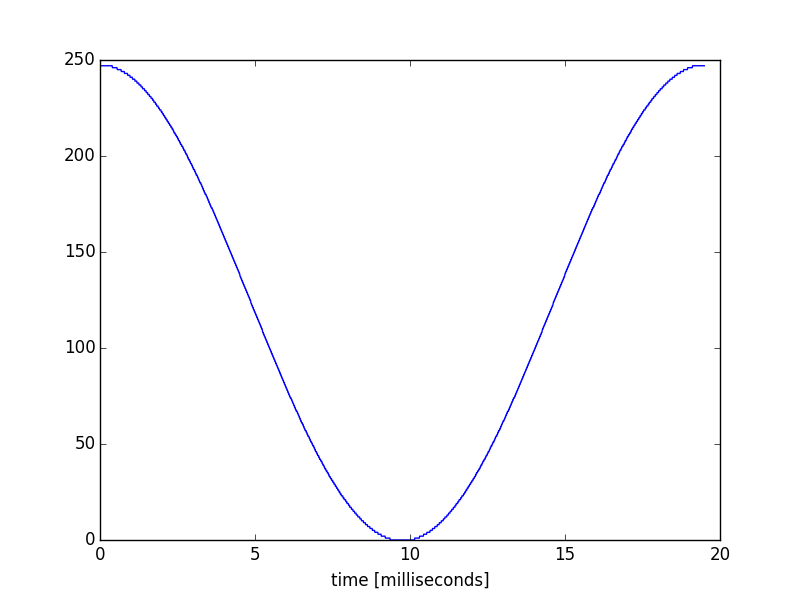
\includegraphics[width=0.75\textwidth]{figs/waveform.png}}
\end{center}
\caption{\label{fig:wave} Test pattern from Arduino plotted in Scientific Python.}
\end{figure}


\section{Periodogram}

An example ipython notebook using scientific python to create a periodogram is also available on the course website.  First, a test pattern (sine wave) is filled as shown in Fig.~\ref{fig:testpatterns}.  Then the periodogram is calculated and plotted as in Fig.~\ref{fig:periodogram}.

\begin{figure}[htbp]
\begin{center}
{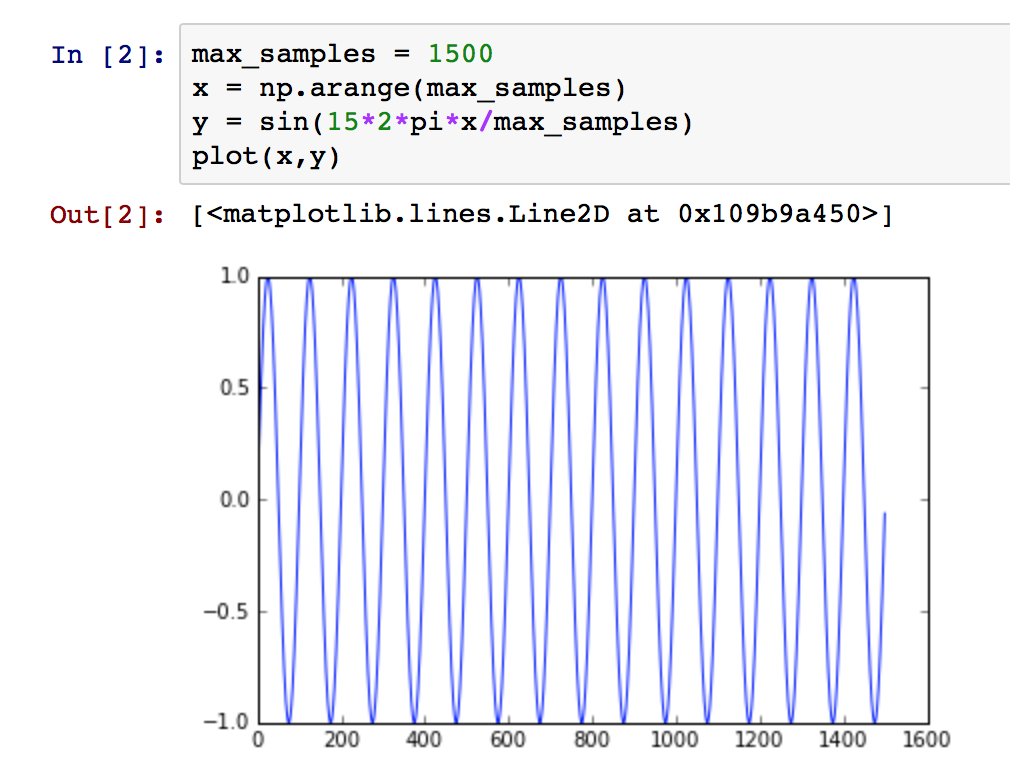
\includegraphics[width=0.65\textwidth]{figs/testpattern.png}}
\end{center}
\caption{\label{fig:testpattern} Creating a test pattern for the periodogram.}
\end{figure}

\begin{figure}[htbp]
\begin{center}
{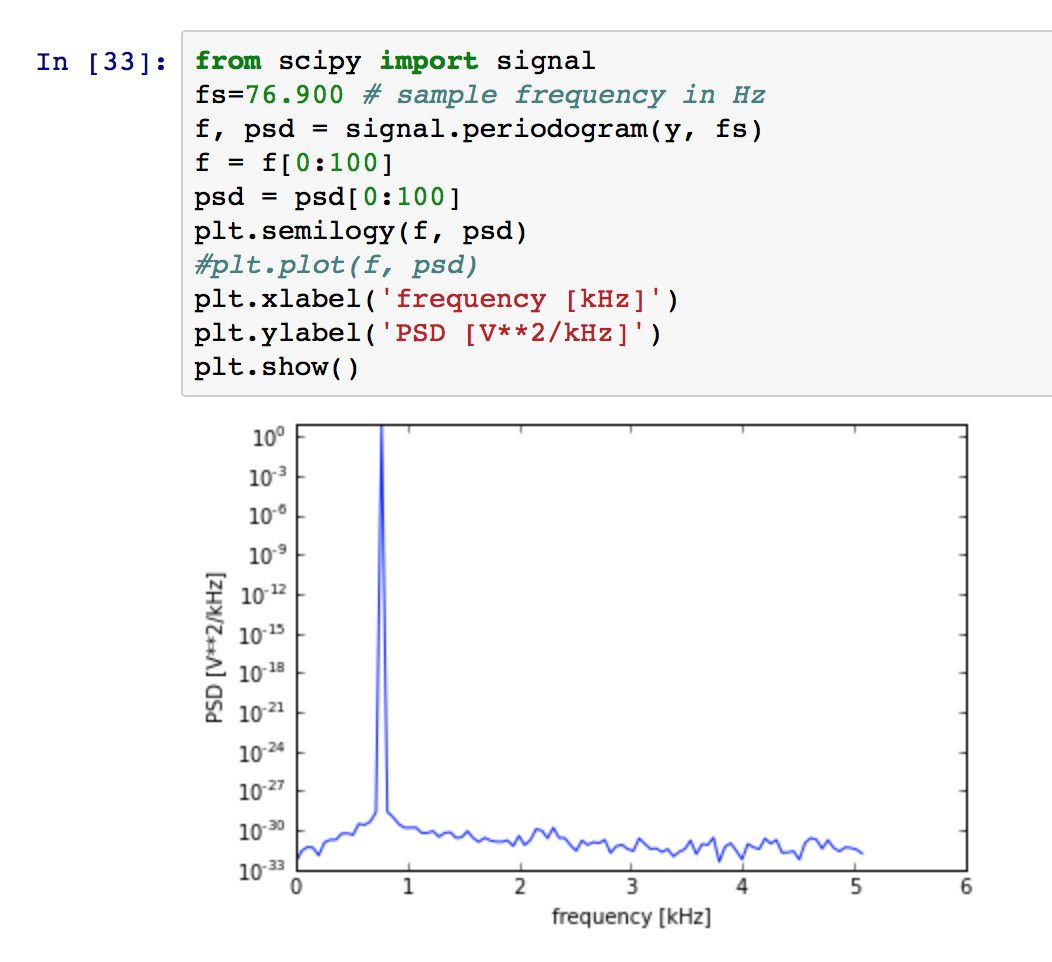
\includegraphics[width=0.65\textwidth]{figs/periodogram.png}}
\end{center}
\caption{\label{fig:periodogram} Periodogram from test pattern.}
\end{figure}




\section{Improvements}

There are several possible improvements that you can pursue if you have time.\\

\noindent
{\bf Frequency Resolution:}  We worked hard to get the ADC sampling rate as high as possible.  But, we are limited to about 1500 samples, and this limits our sampling period to about $19.5~\rm ms$ and our frequency resolution ($f_1$) to about $50~\rm Hz$.  That's enough to tell the difference between guitar strings, but not to tune them.

One way around this would be to simply lower the sampling rate.  As long as we keep the Nyquist rate above $10~\rm kHz$ (where the microphone cuts out) we don't have to worry about aliasing.  So we could simply skip two out of every three samples, increasing our frequency resolution to $16~\rm Hz$.

But there's something better we can do.  If we simply average $n$ samples and save that to the buffer, we produce, effectively a low-pass filter with a very sharp cutoff.  We are still sampling at the higher rate, so the Nyquist frequency remains comfortable high at around $30~\rm kHz$.  Averaging samples kills any frequency component between $30~\rm kHz$ and the Nyquist frequency for the reduced sampling rate.\\

\noindent
{\bf Boosting Signal To Noise:}  Averaging the periodograms from several waveforms should increase the signal to noise ratio by eliminating random noise.  The driver interface already includes a parameter (currently set to one) for the number of buffers to send.

\end{document}


